\pgfdeclareplotmark{cross} {
\pgfpathmoveto{\pgfpoint{-0.3\pgfplotmarksize}{\pgfplotmarksize}}
\pgfpathlineto{\pgfpoint{+0.3\pgfplotmarksize}{\pgfplotmarksize}}
\pgfpathlineto{\pgfpoint{+0.3\pgfplotmarksize}{0.3\pgfplotmarksize}}
\pgfpathlineto{\pgfpoint{+1\pgfplotmarksize}{0.3\pgfplotmarksize}}
\pgfpathlineto{\pgfpoint{+1\pgfplotmarksize}{-0.3\pgfplotmarksize}}
\pgfpathlineto{\pgfpoint{+0.3\pgfplotmarksize}{-0.3\pgfplotmarksize}}
\pgfpathlineto{\pgfpoint{+0.3\pgfplotmarksize}{-1.\pgfplotmarksize}}
\pgfpathlineto{\pgfpoint{-0.3\pgfplotmarksize}{-1.\pgfplotmarksize}}
\pgfpathlineto{\pgfpoint{-0.3\pgfplotmarksize}{-0.3\pgfplotmarksize}}
\pgfpathlineto{\pgfpoint{-1.\pgfplotmarksize}{-0.3\pgfplotmarksize}}
\pgfpathlineto{\pgfpoint{-1.\pgfplotmarksize}{0.3\pgfplotmarksize}}
\pgfpathlineto{\pgfpoint{-0.3\pgfplotmarksize}{0.3\pgfplotmarksize}}
\pgfpathclose
\pgfusepathqstroke
}
\pgfdeclareplotmark{cross*} {
\pgfpathmoveto{\pgfpoint{-0.3\pgfplotmarksize}{\pgfplotmarksize}}
\pgfpathlineto{\pgfpoint{+0.3\pgfplotmarksize}{\pgfplotmarksize}}
\pgfpathlineto{\pgfpoint{+0.3\pgfplotmarksize}{0.3\pgfplotmarksize}}
\pgfpathlineto{\pgfpoint{+1\pgfplotmarksize}{0.3\pgfplotmarksize}}
\pgfpathlineto{\pgfpoint{+1\pgfplotmarksize}{-0.3\pgfplotmarksize}}
\pgfpathlineto{\pgfpoint{+0.3\pgfplotmarksize}{-0.3\pgfplotmarksize}}
\pgfpathlineto{\pgfpoint{+0.3\pgfplotmarksize}{-1.\pgfplotmarksize}}
\pgfpathlineto{\pgfpoint{-0.3\pgfplotmarksize}{-1.\pgfplotmarksize}}
\pgfpathlineto{\pgfpoint{-0.3\pgfplotmarksize}{-0.3\pgfplotmarksize}}
\pgfpathlineto{\pgfpoint{-1.\pgfplotmarksize}{-0.3\pgfplotmarksize}}
\pgfpathlineto{\pgfpoint{-1.\pgfplotmarksize}{0.3\pgfplotmarksize}}
\pgfpathlineto{\pgfpoint{-0.3\pgfplotmarksize}{0.3\pgfplotmarksize}}
\pgfpathclose
\pgfusepathqfillstroke
}
\pgfdeclareplotmark{newstar} {
\pgfpathmoveto{\pgfqpoint{0pt}{\pgfplotmarksize}}
\pgfpathlineto{\pgfqpointpolar{44}{0.5\pgfplotmarksize}}
\pgfpathlineto{\pgfqpointpolar{18}{\pgfplotmarksize}}
\pgfpathlineto{\pgfqpointpolar{-20}{0.5\pgfplotmarksize}}
\pgfpathlineto{\pgfqpointpolar{-54}{\pgfplotmarksize}}
\pgfpathlineto{\pgfqpointpolar{-90}{0.5\pgfplotmarksize}}
\pgfpathlineto{\pgfqpointpolar{234}{\pgfplotmarksize}}
\pgfpathlineto{\pgfqpointpolar{198}{0.5\pgfplotmarksize}}
\pgfpathlineto{\pgfqpointpolar{162}{\pgfplotmarksize}}
\pgfpathlineto{\pgfqpointpolar{134}{0.5\pgfplotmarksize}}
\pgfpathclose
\pgfusepathqstroke
}
\pgfdeclareplotmark{newstar*} {
\pgfpathmoveto{\pgfqpoint{0pt}{\pgfplotmarksize}}
\pgfpathlineto{\pgfqpointpolar{44}{0.5\pgfplotmarksize}}
\pgfpathlineto{\pgfqpointpolar{18}{\pgfplotmarksize}}
\pgfpathlineto{\pgfqpointpolar{-20}{0.5\pgfplotmarksize}}
\pgfpathlineto{\pgfqpointpolar{-54}{\pgfplotmarksize}}
\pgfpathlineto{\pgfqpointpolar{-90}{0.5\pgfplotmarksize}}
\pgfpathlineto{\pgfqpointpolar{234}{\pgfplotmarksize}}
\pgfpathlineto{\pgfqpointpolar{198}{0.5\pgfplotmarksize}}
\pgfpathlineto{\pgfqpointpolar{162}{\pgfplotmarksize}}
\pgfpathlineto{\pgfqpointpolar{134}{0.5\pgfplotmarksize}}
\pgfpathclose
\pgfusepathqfillstroke
}
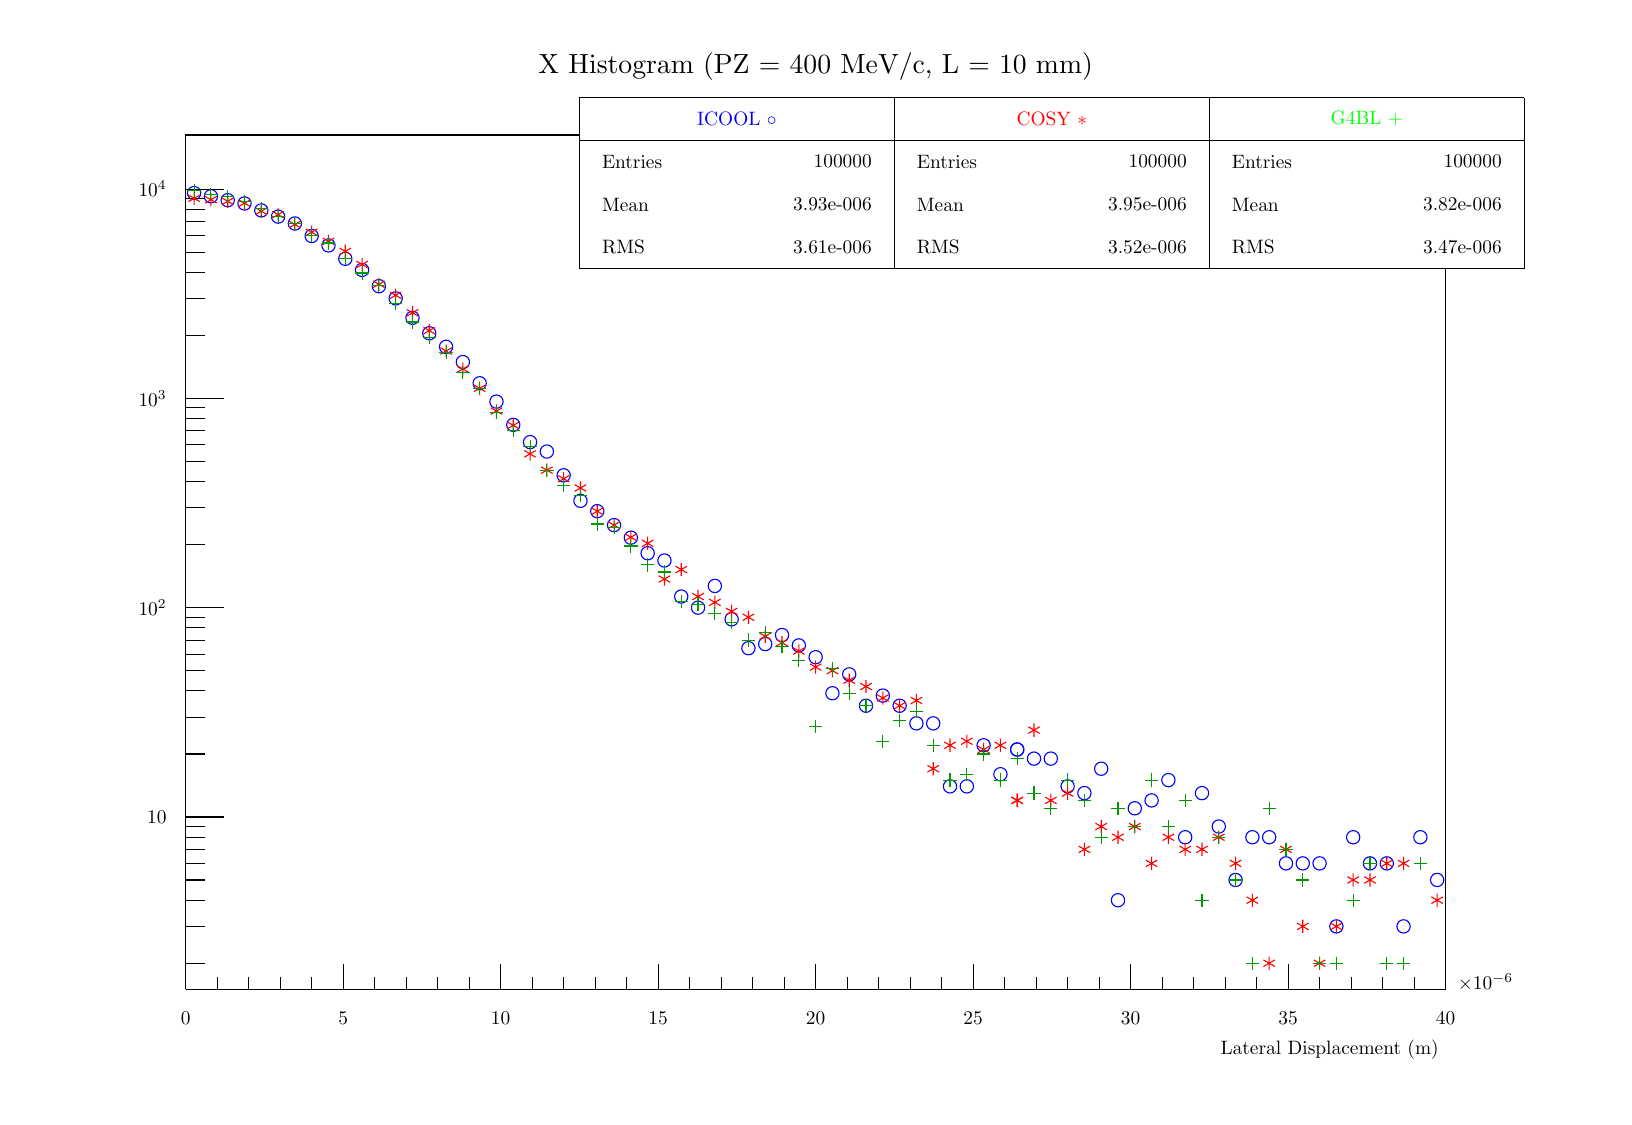
\begin{tikzpicture}
\definecolor{c}{rgb}{1,1,1};
\draw [color=c, fill=c] (0,0) rectangle (20,13.5632);
\draw [color=c, fill=c] (2,1.35632) rectangle (18,12.2069);
\definecolor{c}{rgb}{0,0,0};
\draw [c] (2,1.35632) -- (2,12.2069) -- (18,12.2069) -- (18,1.35632) -- (2,1.35632);
\definecolor{c}{rgb}{1,1,1};
\draw [color=c, fill=c] (2,1.35632) rectangle (18,12.2069);
\definecolor{c}{rgb}{0,0,0};
\draw [c] (2,1.35632) -- (2,12.2069) -- (18,12.2069) -- (18,1.35632) -- (2,1.35632);
\definecolor{c}{rgb}{0,0,1};
\foreach \P in
 {(2.10667,11.4692),(2.32,11.4286),(2.53333,11.3794),(2.74667,11.3377),(2.96,11.2494),(3.17333,11.1705),(3.38667,11.083),(3.6,10.9243),(3.81333,10.8048),(4.02667,10.635),(4.24,10.4937),(4.45333,10.2872),(4.66667,10.1313),(4.88,9.8854),(5.09333,9.6893
1),(5.30667,9.5169),(5.52,9.32346),(5.73333,9.0544),(5.94667,8.82123),(6.16,8.52564),(6.37333,8.3068),(6.58667,8.18683),(6.8,7.88541),(7.01333,7.56137),(7.22667,7.4294),(7.44,7.25279),(7.65333,7.09331),(7.86667,6.8956),(8.08,6.8032),(8.29333,6.34541)
,(8.50667,6.20432),(8.72,6.48024),(8.93333,6.05676),(9.14667,5.68915),(9.36,5.74203),(9.57333,5.85674),(9.78667,5.72467),(10,5.57551),(10.2133,5.11736),(10.4267,5.35705),(10.64,4.95898),(10.8533,5.08738),(11.0667,4.95898),(11.28,4.73485),(11.4933,4.7
3485),(11.7067,3.93471),(11.92,3.93471),(12.1333,4.45646),(12.3467,4.08885),(12.56,4.40276)}{\draw[mark options={color=c,fill=c},mark size=2.402402pt,mark=o] plot coordinates {\P};}
\foreach \P in
 {(12.56,4.40276),(12.7733,4.28723),(12.9867,4.28723),(13.2,3.93471),(13.4133,3.84916),(13.6267,4.15883),(13.84,2.48856),(14.0533,3.65632),(14.2667,3.75676),(14.48,4.01435),(14.6933,3.28871),(14.9067,3.84916),(15.12,3.42467),(15.3333,2.74615),(15.546
7,3.28871),(15.76,3.28871),(15.9733,2.95661),(16.1867,2.95661),(16.4,2.95661),(16.6133,2.15647),(16.8267,3.28871),(17.04,2.95661),(17.2533,2.95661),(17.4667,2.15647),(17.68,3.28871),(17.8933,2.74615)}{\draw[mark options={color=c,fill=c},mark
 size=2.402402pt,mark=o] plot coordinates {\P};}
\definecolor{c}{rgb}{1,1,1};
\draw [color=c, fill=c] (7,10.5115) rectangle (11,12.6816);
\definecolor{c}{rgb}{0,0,0};
\draw [c] (7,10.5115) -- (11,10.5115);
\draw [c] (11,10.5115) -- (11,12.6816);
\draw [c] (11,12.6816) -- (7,12.6816);
\draw [c] (7,12.6816) -- (7,10.5115);
\draw[color=blue](9,12.4103) node[scale=0.7, rotate=0]{ICOOL $\circ$};
\draw [c] (7,12.1391) -- (11,12.1391);
\draw [anchor= west] (7.2,11.8678) node[scale=0.7, rotate=0]{Entries };
\draw [anchor= east] (10.8,11.8678) node[scale=0.7, rotate=0]{ 100000};
\draw [anchor= west] (7.2,11.3253) node[scale=0.7, rotate=0]{Mean  };
\draw [anchor= east] (10.8,11.3253) node[scale=0.7, rotate=0]{ 3.93e-006};
\draw [anchor= west] (7.2,10.7828) node[scale=0.7, rotate=0]{RMS   };
\draw [anchor= east] (10.8,10.7828) node[scale=0.7, rotate=0]{ 3.61e-006};
\draw [c] (2,1.35632) -- (18,1.35632);
\draw [anchor= east] (18,0.596782) node[scale=0.7, rotate=0]{Lateral Displacement (m)};
\draw [c] (2,1.68184) -- (2,1.35632);
\draw [c] (2.4,1.51908) -- (2.4,1.35632);
\draw [c] (2.8,1.51908) -- (2.8,1.35632);
\draw [c] (3.2,1.51908) -- (3.2,1.35632);
\draw [c] (3.6,1.51908) -- (3.6,1.35632);
\draw [c] (4,1.68184) -- (4,1.35632);
\draw [c] (4.4,1.51908) -- (4.4,1.35632);
\draw [c] (4.8,1.51908) -- (4.8,1.35632);
\draw [c] (5.2,1.51908) -- (5.2,1.35632);
\draw [c] (5.6,1.51908) -- (5.6,1.35632);
\draw [c] (6,1.68184) -- (6,1.35632);
\draw [c] (6.4,1.51908) -- (6.4,1.35632);
\draw [c] (6.8,1.51908) -- (6.8,1.35632);
\draw [c] (7.2,1.51908) -- (7.2,1.35632);
\draw [c] (7.6,1.51908) -- (7.6,1.35632);
\draw [c] (8,1.68184) -- (8,1.35632);
\draw [c] (8.4,1.51908) -- (8.4,1.35632);
\draw [c] (8.8,1.51908) -- (8.8,1.35632);
\draw [c] (9.2,1.51908) -- (9.2,1.35632);
\draw [c] (9.6,1.51908) -- (9.6,1.35632);
\draw [c] (10,1.68184) -- (10,1.35632);
\draw [c] (10.4,1.51908) -- (10.4,1.35632);
\draw [c] (10.8,1.51908) -- (10.8,1.35632);
\draw [c] (11.2,1.51908) -- (11.2,1.35632);
\draw [c] (11.6,1.51908) -- (11.6,1.35632);
\draw [c] (12,1.68184) -- (12,1.35632);
\draw [c] (12.4,1.51908) -- (12.4,1.35632);
\draw [c] (12.8,1.51908) -- (12.8,1.35632);
\draw [c] (13.2,1.51908) -- (13.2,1.35632);
\draw [c] (13.6,1.51908) -- (13.6,1.35632);
\draw [c] (14,1.68184) -- (14,1.35632);
\draw [c] (14.4,1.51908) -- (14.4,1.35632);
\draw [c] (14.8,1.51908) -- (14.8,1.35632);
\draw [c] (15.2,1.51908) -- (15.2,1.35632);
\draw [c] (15.6,1.51908) -- (15.6,1.35632);
\draw [c] (16,1.68184) -- (16,1.35632);
\draw [c] (16.4,1.51908) -- (16.4,1.35632);
\draw [c] (16.8,1.51908) -- (16.8,1.35632);
\draw [c] (17.2,1.51908) -- (17.2,1.35632);
\draw [c] (17.6,1.51908) -- (17.6,1.35632);
\draw [c] (18,1.68184) -- (18,1.35632);
\draw [anchor=base] (2,0.908736) node[scale=0.7, rotate=0]{0};
\draw [anchor=base] (4,0.908736) node[scale=0.7, rotate=0]{5};
\draw [anchor=base] (6,0.908736) node[scale=0.7, rotate=0]{10};
\draw [anchor=base] (8,0.908736) node[scale=0.7, rotate=0]{15};
\draw [anchor=base] (10,0.908736) node[scale=0.7, rotate=0]{20};
\draw [anchor=base] (12,0.908736) node[scale=0.7, rotate=0]{25};
\draw [anchor=base] (14,0.908736) node[scale=0.7, rotate=0]{30};
\draw [anchor=base] (16,0.908736) node[scale=0.7, rotate=0]{35};
\draw [anchor=base] (18,0.908736) node[scale=0.7, rotate=0]{40};
\draw [anchor=base west] (18.07,1.35632) node[scale=0.7, rotate=0]{$\times10^{-6}$};
\draw [c] (2,1.35632) -- (2,12.2069);
\draw [c] (2.24,1.68841) -- (2,1.68841);
\draw [c] (2.24,2.15647) -- (2,2.15647);
\draw [c] (2.24,2.48856) -- (2,2.48856);
\draw [c] (2.24,2.74615) -- (2,2.74615);
\draw [c] (2.24,2.95661) -- (2,2.95661);
\draw [c] (2.24,3.13456) -- (2,3.13456);
\draw [c] (2.24,3.2887) -- (2,3.2887);
\draw [c] (2.24,3.42467) -- (2,3.42467);
\draw [c] (2.48,3.54629) -- (2,3.54629);
\draw [anchor= east] (1.844,3.54629) node[scale=0.7, rotate=0]{10};
\draw [c] (2.24,4.34644) -- (2,4.34644);
\draw [c] (2.24,4.8145) -- (2,4.8145);
\draw [c] (2.24,5.14659) -- (2,5.14659);
\draw [c] (2.24,5.40418) -- (2,5.40418);
\draw [c] (2.24,5.61464) -- (2,5.61464);
\draw [c] (2.24,5.79259) -- (2,5.79259);
\draw [c] (2.24,5.94673) -- (2,5.94673);
\draw [c] (2.24,6.0827) -- (2,6.0827);
\draw [c] (2.48,6.20432) -- (2,6.20432);
\draw [anchor= east] (1.844,6.20432) node[scale=0.7, rotate=0]{$10^{2}$};
\draw [c] (2.24,7.00447) -- (2,7.00447);
\draw [c] (2.24,7.47253) -- (2,7.47253);
\draw [c] (2.24,7.80462) -- (2,7.80462);
\draw [c] (2.24,8.06221) -- (2,8.06221);
\draw [c] (2.24,8.27267) -- (2,8.27267);
\draw [c] (2.24,8.45062) -- (2,8.45062);
\draw [c] (2.24,8.60476) -- (2,8.60476);
\draw [c] (2.24,8.74073) -- (2,8.74073);
\draw [c] (2.48,8.86235) -- (2,8.86235);
\draw [anchor= east] (1.844,8.86235) node[scale=0.7, rotate=0]{$10^{3}$};
\draw [c] (2.24,9.6625) -- (2,9.6625);
\draw [c] (2.24,10.1306) -- (2,10.1306);
\draw [c] (2.24,10.4626) -- (2,10.4626);
\draw [c] (2.24,10.7202) -- (2,10.7202);
\draw [c] (2.24,10.9307) -- (2,10.9307);
\draw [c] (2.24,11.1086) -- (2,11.1086);
\draw [c] (2.24,11.2628) -- (2,11.2628);
\draw [c] (2.24,11.3988) -- (2,11.3988);
\draw [c] (2.48,11.5204) -- (2,11.5204);
\draw [anchor= east] (1.844,11.5204) node[scale=0.7, rotate=0]{$10^{4}$};
\definecolor{c}{rgb}{1,1,1};
\draw [color=c, fill=c] (7,10.5115) rectangle (11,12.6816);
\definecolor{c}{rgb}{0,0,0};
\draw [c] (7,10.5115) -- (11,10.5115);
\draw [c] (11,10.5115) -- (11,12.6816);
\draw [c] (11,12.6816) -- (7,12.6816);
\draw [c] (7,12.6816) -- (7,10.5115);
\draw[color=blue](9,12.4103) node[scale=0.7, rotate=0]{ICOOL $\circ$};
\draw [c] (7,12.1391) -- (11,12.1391);
\draw [anchor= west] (7.2,11.8678) node[scale=0.7, rotate=0]{Entries };
\draw [anchor= east] (10.8,11.8678) node[scale=0.7, rotate=0]{ 100000};
\draw [anchor= west] (7.2,11.3253) node[scale=0.7, rotate=0]{Mean  };
\draw [anchor= east] (10.8,11.3253) node[scale=0.7, rotate=0]{ 3.93e-006};
\draw [anchor= west] (7.2,10.7828) node[scale=0.7, rotate=0]{RMS   };
\draw [anchor= east] (10.8,10.7828) node[scale=0.7, rotate=0]{ 3.61e-006};
\draw (10,13.0816) node[scale=1, rotate=0]{X Histogram (PZ = 400 MeV/c, L = 10 mm)};
\definecolor{c}{rgb}{1,0,0};
\foreach \P in
 {(2.10667,11.4029),(2.32,11.3851),(2.53333,11.366),(2.74667,11.341),(2.96,11.2398),(3.17333,11.1957),(3.38667,11.0709),(3.6,10.9728),(3.81333,10.856),(4.02667,10.729),(4.24,10.5624),(4.45333,10.3115),(4.66667,10.171),(4.88,9.94927),(5.09333,9.72212)
,(5.30667,9.46329),(5.52,9.23499),(5.73333,8.99008),(5.94667,8.70159),(6.16,8.51944),(6.37333,8.15744),(6.58667,7.9508),(6.8,7.84154),(7.01333,7.72394),(7.22667,7.4294),(7.44,7.25279),(7.65333,7.09864),(7.86667,7.02166),(8.08,6.56773),(8.29333,6.6876
7),(8.50667,6.34541),(8.72,6.27159),(8.93333,6.1572),(9.14667,6.0827),(9.36,5.84103),(9.57333,5.75913),(9.78667,5.6525),(10,5.44945),(10.2133,5.40418),(10.4267,5.28255),(10.64,5.20291),(10.8533,5.05659),(11.0667,4.95898),(11.28,5.02496),(11.4933,4.15
883),(11.7067,4.45646),(11.92,4.50778),(12.1333,4.40276),(12.3467,4.45646),(12.56,3.75676)}{\draw[mark options={color=c,fill=c},mark size=2.402402pt,mark=asterisk] plot coordinates {\P};}
\foreach \P in
 {(12.56,3.75676),(12.7733,4.64931),(12.9867,3.75676),(13.2,3.84916),(13.4133,3.13456),(13.6267,3.42467),(13.84,3.28871),(14.0533,3.42467),(14.2667,2.95661),(14.48,3.28871),(14.6933,3.13456),(14.9067,3.13456),(15.12,3.28871),(15.3333,2.95661),(15.546
7,2.48856),(15.76,1.68841),(15.9733,3.13456),(16.1867,2.15647),(16.4,1.68841),(16.6133,2.15647),(16.8267,2.74615),(17.04,2.74615),(17.2533,2.95661),(17.4667,2.95661),(17.8933,2.48856)}{\draw[mark options={color=c,fill=c},mark
 size=2.402402pt,mark=asterisk] plot coordinates {\P};}
\definecolor{c}{rgb}{1,1,1};
\draw [color=c, fill=c] (11,10.5115) rectangle (15,12.6816);
\definecolor{c}{rgb}{0,0,0};
\draw [c] (11,10.5115) -- (15,10.5115);
\draw [c] (15,10.5115) -- (15,12.6816);
\draw [c] (15,12.6816) -- (11,12.6816);
\draw [c] (11,12.6816) -- (11,10.5115);
\draw [color=red](13,12.4103) node[scale=0.7, rotate=0]{COSY $*$};
\draw [c] (11,12.1391) -- (15,12.1391);
\draw [anchor= west] (11.2,11.8678) node[scale=0.7, rotate=0]{Entries };
\draw [anchor= east] (14.8,11.8678) node[scale=0.7, rotate=0]{ 100000};
\draw [anchor= west] (11.2,11.3253) node[scale=0.7, rotate=0]{Mean  };
\draw [anchor= east] (14.8,11.3253) node[scale=0.7, rotate=0]{ 3.95e-006};
\draw [anchor= west] (11.2,10.7828) node[scale=0.7, rotate=0]{RMS   };
\draw [anchor= east] (14.8,10.7828) node[scale=0.7, rotate=0]{ 3.52e-006};
\definecolor{c}{rgb}{1,1,1};
\draw [color=c, fill=c] (11,10.5115) rectangle (15,12.6816);
\definecolor{c}{rgb}{0,0,0};
\draw [c] (11,10.5115) -- (15,10.5115);
\draw [c] (15,10.5115) -- (15,12.6816);
\draw [c] (15,12.6816) -- (11,12.6816);
\draw [c] (11,12.6816) -- (11,10.5115);
\draw [color=red](13,12.4103) node[scale=0.7, rotate=0]{COSY $*$};
\draw [c] (11,12.1391) -- (15,12.1391);
\draw [anchor= west] (11.2,11.8678) node[scale=0.7, rotate=0]{Entries };
\draw [anchor= east] (14.8,11.8678) node[scale=0.7, rotate=0]{ 100000};
\draw [anchor= west] (11.2,11.3253) node[scale=0.7, rotate=0]{Mean  };
\draw [anchor= east] (14.8,11.3253) node[scale=0.7, rotate=0]{ 3.95e-006};
\draw [anchor= west] (11.2,10.7828) node[scale=0.7, rotate=0]{RMS   };
\draw [anchor= east] (14.8,10.7828) node[scale=0.7, rotate=0]{ 3.52e-006};
\definecolor{c}{rgb}{0,0.6,0};
\foreach \P in
 {(2.10667,11.4967),(2.32,11.4528),(2.53333,11.4286),(2.74667,11.3636),(2.96,11.2708),(3.17333,11.1751),(3.38667,11.0858),(3.6,10.9363),(3.81333,10.8357),(4.02667,10.6407),(4.24,10.4542),(4.45333,10.2996),(4.66667,10.0705),(4.88,9.83184),(5.09333,9.6
3859),(5.30667,9.44392),(5.52,9.19242),(5.73333,8.99111),(5.94667,8.67881),(6.16,8.45062),(6.37333,8.24739),(6.58667,7.9457),(6.8,7.75749),(7.01333,7.63051),(7.22667,7.26667),(7.44,7.22452),(7.65333,6.98702),(7.86667,6.74688),(8.08,6.65688),(8.29333,
6.28243),(8.50667,6.2496),(8.72,6.1329),(8.93333,6.01672),(9.14667,5.79259),(9.36,5.88752),(9.57333,5.70704),(9.78667,5.535),(10,4.69287),(10.2133,5.42704),(10.4267,5.11736),(10.64,4.95898),(10.8533,4.50778),(11.0667,4.77536),(11.28,4.889),(11.4933,4
.45646),(11.7067,4.01435),(11.92,4.08885),(12.1333,4.34644),(12.3467,4.01435),(12.56,4.28723)}{\draw[mark options={color=c,fill=c},mark size=2.402402pt,mark=+] plot coordinates {\P};}
\foreach \P in
 {(12.56,4.28723),(12.7733,3.84916),(12.9867,3.65632),(13.2,4.01435),(13.4133,3.75676),(13.6267,3.28871),(13.84,3.65632),(14.0533,3.42467),(14.2667,4.01435),(14.48,3.42467),(14.6933,3.75676),(14.9067,2.48856),(15.12,3.28871),(15.3333,2.74615),(15.546
7,1.68841),(15.76,3.65632),(15.9733,3.13456),(16.1867,2.74615),(16.4,1.68841),(16.6133,1.68841),(16.8267,2.48856),(17.04,2.95661),(17.2533,1.68841),(17.4667,1.68841),(17.68,2.95661)}{\draw[mark options={color=c,fill=c},mark size=2.402402pt,mark=+]
 plot coordinates {\P};}
\definecolor{c}{rgb}{1,1,1};
\draw [color=c, fill=c] (15,10.5115) rectangle (19,12.6816);
\definecolor{c}{rgb}{0,0,0};
\draw [c] (15,10.5115) -- (19,10.5115);
\draw [c] (19,10.5115) -- (19,12.6816);
\draw [c] (19,12.6816) -- (15,12.6816);
\draw [c] (15,12.6816) -- (15,10.5115);
\draw [color=green](17,12.4103) node[scale=0.7, rotate=0]{G4BL $+$};
\draw [c] (15,12.1391) -- (19,12.1391);
\draw [anchor= west] (15.2,11.8678) node[scale=0.7, rotate=0]{Entries };
\draw [anchor= east] (18.8,11.8678) node[scale=0.7, rotate=0]{ 100000};
\draw [anchor= west] (15.2,11.3253) node[scale=0.7, rotate=0]{Mean  };
\draw [anchor= east] (18.8,11.3253) node[scale=0.7, rotate=0]{ 3.82e-006};
\draw [anchor= west] (15.2,10.7828) node[scale=0.7, rotate=0]{RMS   };
\draw [anchor= east] (18.8,10.7828) node[scale=0.7, rotate=0]{ 3.47e-006};
\definecolor{c}{rgb}{1,1,1};
\draw [color=c, fill=c] (15,10.5115) rectangle (19,12.6816);
\definecolor{c}{rgb}{0,0,0};
\draw [c] (15,10.5115) -- (19,10.5115);
\draw [c] (19,10.5115) -- (19,12.6816);
\draw [c] (19,12.6816) -- (15,12.6816);
\draw [c] (15,12.6816) -- (15,10.5115);
\draw [color=green](17,12.4103) node[scale=0.7, rotate=0]{G4BL $+$};
\draw [c] (15,12.1391) -- (19,12.1391);
\draw [anchor= west] (15.2,11.8678) node[scale=0.7, rotate=0]{Entries };
\draw [anchor= east] (18.8,11.8678) node[scale=0.7, rotate=0]{ 100000};
\draw [anchor= west] (15.2,11.3253) node[scale=0.7, rotate=0]{Mean  };
\draw [anchor= east] (18.8,11.3253) node[scale=0.7, rotate=0]{ 3.82e-006};
\draw [anchor= west] (15.2,10.7828) node[scale=0.7, rotate=0]{RMS   };
\draw [anchor= east] (18.8,10.7828) node[scale=0.7, rotate=0]{ 3.47e-006};
\end{tikzpicture}
